\documentclass[conference]{IEEEtran}

\usepackage{amsmath,amssymb,amsfonts}
\usepackage{graphicx}
\usepackage{textcomp}
\usepackage{xcolor}
\usepackage{booktabs}
\usepackage{listings}
\usepackage{url}
\usepackage{hyperref}
\usepackage{cite}

\lstset{
    language=Python,
    basicstyle=\ttfamily\footnotesize,
    keywordstyle=\color{blue}\bfseries,
    commentstyle=\color{gray}\itshape,
    stringstyle=\color{red},
    numbers=left,
    numberstyle=\tiny\color{gray},
    numbersep=5pt,
    frame=single,
    breaklines=true,
    captionpos=b,
    tabsize=4
}

\def\BibTeX{{\rm B\kern-.05em{\sc i\kern-.025em b}\kern-.08em
        T\kern-.1667em\lower.7ex\hbox{E}\kern-.125emX}}

\begin{document}

\title{Market Basket Analysis on Online Retail Data:\\
A Comparative Study of Apriori and FP-Growth Algorithms\\
with Multi-Measure Rule Evaluation\\
{\footnotesize BIL 476 / 573 --- Data Mining Course Project, Spring 2026\\
    TOBB University of Economics and Technology}
}

\author{\IEEEauthorblockN{Erdem Baran}
    \IEEEauthorblockA{\textit{TOBB University of Economics and Technology}\\
        Ankara, Turkey \\
        Student ID: 211101034 \\
        ebaran@etu.edu.tr}
}

\maketitle

\begin{abstract}
In this project, I applied market basket analysis to the UCI Online Retail dataset, which contains 541,909 transaction records from a UK-based online retailer collected between December 2010 and December 2011. After cleaning the data, I worked with 396,470 records and built a transaction matrix of 16,579 baskets across 3,828 unique products. I compared two well-known algorithms, Apriori and FP-Growth, to see which one finds frequent itemsets faster and how they scale when the support threshold changes. Both algorithms found the same 239 frequent itemsets at 2\% support, but FP-Growth was up to 30 times faster at lower thresholds. I then evaluated the rules using five measures: support, confidence, lift, Kulczynski, and cosine. The most interesting rule connected the three-piece Regency Teacup and Saucer set, with a lift of 24.12. I also found that lift and support are almost uncorrelated (r = -0.014), which means that popular items are not always the most interesting ones. This project showed me how much the choice of algorithm and evaluation measure matters in practice.
\end{abstract}

\begin{IEEEkeywords}
market basket analysis, association rule mining, Apriori, FP-Growth, interestingness measures
\end{IEEEkeywords}

% -------------------------------------------------------
\section{Introduction}
\label{sec:introduction}

Have you ever wondered why online stores suggest products you did not even search for? A big part of the answer comes from market basket analysis — a data mining technique that looks at which products customers tend to buy together. If many people buy item A and item B in the same order, there is probably a useful relationship between them that a retailer can act on.

In this project, I wanted to find out what kind of purchasing patterns exist in a real online retail dataset and which algorithm discovers them most efficiently. My main research question was: \textit{What meaningful co-purchasing patterns can be found in online retail transaction data, and which algorithm and evaluation measure works best for discovering them?}

To answer this, I used two well-known algorithms: Apriori~\cite{b1} and FP-Growth~\cite{b2}. I applied both to the UCI Online Retail dataset and compared them in terms of runtime and scalability. I also evaluated the discovered rules using five interestingness measures — support, confidence, lift, Kulczynski, and cosine — to understand which ones give the most meaningful results. Kulczynski and cosine are called null-invariant measures, which means they give more reliable results when the dataset is very sparse~\cite{b3}.

The rest of this paper is organized as follows. Section~\ref{sec:related_work} reviews related work. Section~\ref{sec:dataset} describes the dataset. Section~\ref{sec:methodology} explains the steps I followed. Section~\ref{sec:results} presents the findings. Section~\ref{sec:discussion} discusses what the results mean, and Section~\ref{sec:conclusion} summarizes the project.

% -------------------------------------------------------
\section{Related Work}
\label{sec:related_work}

The Apriori algorithm was introduced by Agrawal and Srikant~\cite{b1} in 1994 and quickly became the standard method for finding frequent itemsets. It works by scanning the database multiple times and building up candidate itemsets step by step. The main idea is simple: if an itemset is not frequent, none of its supersets can be frequent either. However, as I found in my experiments, Apriori becomes very slow when the support threshold is low, because the number of candidate itemsets grows very fast.

To solve this problem, Han et al.~\cite{b2} proposed FP-Growth. Instead of generating candidates, FP-Growth compresses all the transactions into a compact tree structure and mines patterns directly from it. This avoids the need for repeated database scans, which is why it is much faster in practice.

One thing I found difficult to understand at first was why confidence alone is not a good measure for evaluating rules. Tan et al.~\cite{b3} explain this clearly: if one item is already very popular, any rule with that item as the consequent will have a high confidence, even if the two items have nothing to do with each other. This is known as the null-invariance problem, and it is why measures like Kulczynski and cosine are useful.

Chen et al.~\cite{b4} used a very similar retail dataset and showed that decisions made during preprocessing — such as how to handle missing values or which transactions to keep — can have a significant impact on the quality of the rules that are found. Their work influenced several choices I made in my own preprocessing pipeline.

Fournier-Viger et al.~\cite{b5} give a broad overview of modern pattern mining techniques. Reading their survey helped me understand the role that classical methods like Apriori and FP-Growth still play today, even though more advanced approaches exist.

% -------------------------------------------------------
\section{Dataset Description}
\label{sec:dataset}

\subsection{Data Source}

I used the UCI Online Retail dataset~\cite{b4}, which is freely available on the UCI Machine Learning Repository at \url{https://archive.ics.uci.edu/dataset/352/online+retail}. It contains all the transactions of a UK-based online shop that sells gifts and homeware items, covering about one year from December 2010 to December 2011.

I chose this dataset because it is a real-world transactional dataset with a good size for market basket analysis. It has more than 500,000 records, 8 attributes of different types, and it covers multiple countries — so it meets all the minimum requirements of the project.

\subsection{Data Characteristics}

Table~\ref{tab:dataset} gives a summary of the main properties. Before any cleaning, the dataset had 541,909 rows. The columns include the invoice number, product code, product description, quantity, date, unit price, customer ID, and country.

\begin{table}[htbp]
    \caption{Dataset Summary}
    \begin{center}
        \begin{tabular}{|l|l|}
            \hline
            \textbf{Property} & \textbf{Value} \\
            \hline
            Total Records (raw) & 541,909 \\
            \hline
            Number of Attributes & 8 \\
            \hline
            Attribute Types & Nominal, Numeric, DateTime \\
            \hline
            Date Range & Dec 2010 -- Dec 2011 \\
            \hline
            Unique Invoices & 25,900 \\
            \hline
            Unique Products (StockCode) & 4,070 \\
            \hline
            Unique Customers & 4,372 \\
            \hline
            Countries & 38 \\
            \hline
            Missing: CustomerID & 135,080 (24.93\%) \\
            \hline
            Missing: Description & 1,454 (0.27\%) \\
            \hline
            Source & UCI ML Repository \\
            \hline
        \end{tabular}
        \label{tab:dataset}
    \end{center}
\end{table}

A few things stood out immediately when I first looked at the data. About 25\% of the rows had no CustomerID, which was a major issue because I needed this field to group items into baskets. The Quantity column had negative values as low as -80,995, which turned out to be product returns. Similarly, UnitPrice had some negative entries that were likely accounting adjustments. Most of the transactions (91.4\%) came from the United Kingdom.

\subsection{Ethical Considerations}

The dataset does not contain any personal information. The CustomerID values are just numbers with no link to real identities. There are no names, addresses, or any other sensitive details. The data is shared publicly by the UCI for research purposes, so there are no ethical concerns with using it in this project.

% -------------------------------------------------------
\section{Methodology}
\label{sec:methodology}

\subsection{Data Preprocessing}

Before running any algorithm, I had to clean the data carefully. I applied five steps, and I will explain the reason behind each one.

\begin{enumerate}
    \item \textbf{Removing cancelled orders:} Invoices starting with the letter ``C'' represent cancellations. There were 9,288 of them. I removed these because a cancelled order does not reflect an actual purchase.
    \item \textbf{Removing rows with missing CustomerID:} There were 134,697 rows without a CustomerID. Since I needed to group transactions by customer to build proper baskets, I had no choice but to remove them.
    \item \textbf{Removing invalid Quantity values:} I removed rows with Quantity $\leq$ 0 to get rid of returns. After the first step, no additional rows were removed here.
    \item \textbf{Removing invalid UnitPrice values:} I removed 40 rows where the price was zero or negative, as these were not real sales.
    \item \textbf{Removing service and test products:} Some rows had stock codes like ``M'', ``D'', or ``POST'' that represent postage fees, bank charges, or manual entries. I removed 1,414 such rows since they are not actual products.
\end{enumerate}

After these steps, 396,470 rows remained (73.2\% of the original). I then focused only on UK transactions, since they make up 91.4\% of the cleaned data. This gave me 354,015 rows and 16,579 unique invoices.

I then built a binary transaction matrix. Each row is one invoice and each column is one product. A cell is 1 if the product appeared in that basket, and 0 otherwise. The resulting matrix was $16,579 \times 3,828$ with a sparsity of 99.5\%, which is normal for retail data. The average basket size was about 20.75 items per invoice.

\subsection{Algorithm Selection and Description}

I chose Apriori and FP-Growth because they represent two very different ways of solving the same problem, and comparing them is a core part of Topic 1.

\textbf{Apriori}~\cite{b1} starts with individual items and builds up to larger itemsets step by step. It uses the fact that if a set is not frequent, none of its supersets can be frequent either. This allows pruning, but the algorithm still needs to scan the database many times, which makes it slow at low support values.

\textbf{FP-Growth}~\cite{b2} avoids candidate generation entirely. It reads the database twice and builds a compressed tree called an FP-tree. It then mines patterns directly from the tree. This is much more efficient, especially when many frequent patterns exist.

I implemented both algorithms using the \texttt{mlxtend} library. The main setting I tested was the minimum support threshold. I used 2\% as the main value and also tested a range from 1\% to 5\% to study scalability.

\subsection{Interestingness Measures}

I evaluated the rules using five measures:

\begin{itemize}
    \item \textbf{Support:} $\text{sup}(A \Rightarrow B) = P(A \cup B)$ — how often the rule appears in the data.
    \item \textbf{Confidence:} $\text{conf}(A \Rightarrow B) = \frac{P(A \cup B)}{P(A)}$ — how often the rule is correct.
    \item \textbf{Lift:} $\text{lift}(A \Rightarrow B) = \frac{P(A \cup B)}{P(A) \cdot P(B)}$ — whether A and B appear together more than by chance.
    \item \textbf{Kulczynski:} $\text{Kulc}(A,B) = \frac{1}{2}\left(\frac{P(A \cup B)}{P(A)} + \frac{P(A \cup B)}{P(B)}\right)$ — a balanced average of the two confidence directions.
    \item \textbf{Cosine (IS):} $\text{cosine}(A,B) = \frac{P(A \cup B)}{\sqrt{P(A) \cdot P(B)}}$ — the geometric mean of the two conditional probabilities.
\end{itemize}

Kulczynski and cosine are null-invariant, meaning they are not affected by how many transactions contain neither A nor B~\cite{b3}. This matters a lot in a sparse dataset like this one.

\subsection{Experimental Setup}

I ran all experiments on my own laptop using Python 3.10 in VS Code with Jupyter Notebook. The libraries I used were \texttt{pandas}, \texttt{numpy}, \texttt{mlxtend 0.23}, \texttt{matplotlib}, and \texttt{seaborn}. Since association rule mining is unsupervised, there was no train/test split. I set a minimum lift of 1.0 to filter out rules where the items appear together no more often than by chance.

% -------------------------------------------------------
\section{Results}
\label{sec:results}

\subsection{Preprocessing Summary}

Table~\ref{tab:preprocessing} shows how many rows were removed at each step. The biggest loss was the missing CustomerID rows — about 25\% of the original data — which is worth keeping in mind when looking at the results.

\begin{table}[htbp]
    \caption{Preprocessing Pipeline Summary}
    \begin{center}
        \begin{tabular}{|l|r|r|}
            \hline
            \textbf{Step} & \textbf{Records Removed} & \textbf{Remaining} \\
            \hline
            Raw data & --- & 541,909 \\
            \hline
            Remove cancellations & 9,288 & 532,621 \\
            \hline
            Remove missing CustomerID & 134,697 & 397,924 \\
            \hline
            Remove invalid Quantity & 0 & 397,924 \\
            \hline
            Remove invalid UnitPrice & 40 & 397,884 \\
            \hline
            Remove service products & 1,414 & 396,470 \\
            \hline
            \textbf{Final (UK only)} & \textbf{---} & \textbf{354,015} \\
            \hline
        \end{tabular}
        \label{tab:preprocessing}
    \end{center}
\end{table}

\subsection{Algorithm Comparison}

At minimum support of 2\%, both Apriori and FP-Growth found exactly the same 239 frequent itemsets, which confirms that both algorithms give correct results. The itemsets included 203 single items, 35 pairs, and 1 triplet. Table~\ref{tab:algo} shows how long each algorithm took at different support values.

\begin{table}[htbp]
    \caption{Apriori vs. FP-Growth Runtime Comparison}
    \begin{center}
        \begin{tabular}{|c|r|r|r|r|}
            \hline
            \textbf{Support} & \textbf{Apriori (s)} & \textbf{FP-Gr. (s)} & \textbf{Speedup} & \textbf{Itemsets} \\
            \hline
            5\% & 0.53 & 1.47 & 0.4$\times$ & 19 \\
            \hline
            4\% & 0.59 & 1.50 & 0.4$\times$ & 44 \\
            \hline
            3\% & 0.82 & 1.74 & 0.5$\times$ & 90 \\
            \hline
            2\% & 3.17 & 1.94 & 1.6$\times$ & 239 \\
            \hline
            1.5\% & 8.01 & 2.16 & 3.7$\times$ & 446 \\
            \hline
            \textbf{1\%} & \textbf{140.97} & \textbf{4.70} & \textbf{30.0$\times$} & \textbf{983} \\
            \hline
        \end{tabular}
        \label{tab:algo}
    \end{center}
\end{table}

What I found quite interesting was that Apriori was actually a bit faster at high support values like 5\% and 4\%. This happens because there are very few frequent itemsets at that level, and the overhead of building the FP-tree is not worth it. But as the threshold dropped to 1\%, Apriori took almost 141 seconds while FP-Growth finished in under 5 seconds — a 30-times difference, which is quite dramatic.

\subsection{Top Association Rules}

I found 76 association rules in total with lift $\geq$ 1 at 2\% support. Table~\ref{tab:toprules} lists the five strongest rules by lift value.

\begin{table}[htbp]
    \caption{Top 5 Association Rules by Lift}
    \begin{center}
        \begin{tabular}{|p{2.2cm}|p{1.8cm}|c|c|c|c|}
            \hline
            \textbf{Antecedent} & \textbf{Consequent} & \textbf{Sup} & \textbf{Conf} & \textbf{Lift} & \textbf{Kulc} \\
            \hline
            GREEN REGENCY TEACUP & PINK+ROSES REGENCY TEACUP & 0.021 & 0.557 & 24.12 & 0.724 \\
            \hline
            PINK REGENCY TEACUP & ROSES+GREEN REGENCY TEACUP & 0.021 & 0.692 & 24.09 & 0.704 \\
            \hline
            GREEN REGENCY TEACUP & PINK REGENCY TEACUP & 0.024 & 0.660 & 22.20 & 0.740 \\
            \hline
            ROSES REGENCY TEACUP & GREEN REGENCY TEACUP & 0.029 & 0.702 & 19.02 & 0.740 \\
            \hline
            GARDENERS KNEELING PAD KEEP CALM & GARDENERS KNEELING PAD CUP OF TEA & 0.028 & 0.617 & 16.32 & 0.674 \\
            \hline
        \end{tabular}
        \label{tab:toprules}
    \end{center}
\end{table}

\subsection{Interestingness Measures Analysis}

Fig.~\ref{fig:scatter} shows the distribution of rules in the support-confidence space (left) and the relationship between Kulczynski and cosine measures (right), with lift encoded as color intensity.

\begin{figure}[htbp]
    \centerline{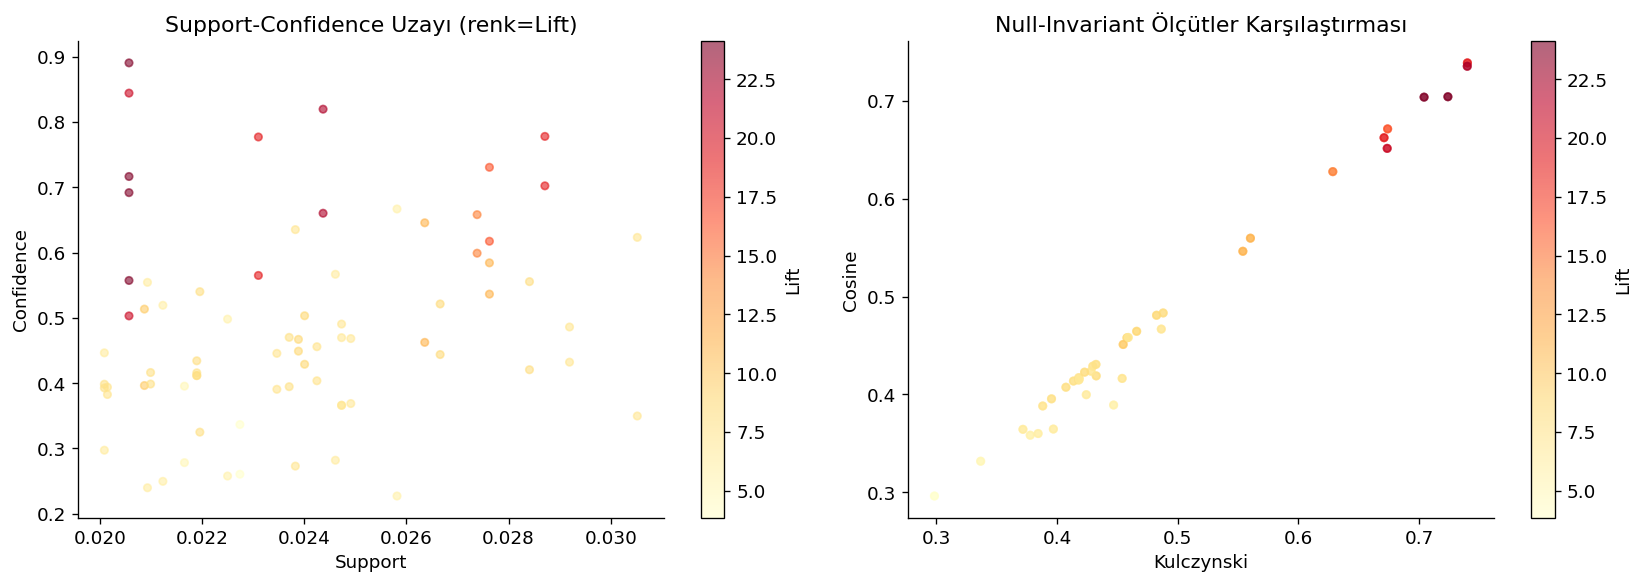
\includegraphics[width=\columnwidth]{rule_measures.png}}
    \caption{Left: Support-Confidence scatter plot colored by lift. Right: Kulczynski vs. Cosine scatter plot. High-lift rules (dark red) cluster at low support but varied confidence levels.}
    \label{fig:scatter}
\end{figure}

Table~\ref{tab:corr} shows the Pearson correlation matrix among all five interestingness measures.

\begin{table}[htbp]
    \caption{Interestingness Measures Correlation Matrix}
    \begin{center}
        \begin{tabular}{|l|c|c|c|c|c|}
            \hline
            & \textbf{Lift} & \textbf{Kulc} & \textbf{Cos} & \textbf{Conf} & \textbf{Sup} \\
            \hline
            \textbf{Lift} & 1.000 & 0.953 & 0.954 & 0.758 & -0.014 \\
            \hline
            \textbf{Kulc} & 0.953 & 1.000 & 0.994 & 0.795 & 0.262 \\
            \hline
            \textbf{Cosine} & 0.954 & 0.994 & 1.000 & 0.791 & 0.264 \\
            \hline
            \textbf{Conf} & 0.758 & 0.795 & 0.791 & 1.000 & 0.208 \\
            \hline
            \textbf{Sup} & -0.014 & 0.262 & 0.264 & 0.208 & 1.000 \\
            \hline
        \end{tabular}
        \label{tab:corr}
    \end{center}
\end{table}

% -------------------------------------------------------
\section{Discussion}
\label{sec:discussion}

\textbf{Which algorithm is better?} Based on my results, FP-Growth is the better choice when the support threshold is low. At 5\% and 4\% support, Apriori was actually a bit faster, because there were very few frequent itemsets and the FP-tree construction was not worth the overhead. But at 1\% support, the difference became enormous — 141 seconds for Apriori versus less than 5 seconds for FP-Growth. In a real company with millions of transactions, running Apriori at a low threshold would simply not be possible.

\textbf{What do the rules mean?} The most interesting patterns I found were all about themed product collections. Customers who buy one colour of the Regency Teacup set almost always buy the others too — the lift value of 24.12 means this is not just a coincidence. The Gardeners Kneeling Pad variants showed a similar pattern (lift = 16.32). From a business point of view, this kind of finding directly supports product bundling and ``you might also like'' recommendation strategies.

\textbf{What did I learn from comparing the measures?} The result that surprised me most was the near-zero correlation between lift and support (r = -0.014). I assumed that popular items would also produce strong rules, but the data showed the opposite. The rules with the highest lift values actually had relatively low support. This means that if you filter rules only by support, you will miss the most interesting patterns completely.

I also noticed that Kulczynski and cosine gave almost identical rankings (r = 0.994), and both agreed closely with lift (r $\approx$ 0.95). This suggests that for this particular dataset, where item frequencies are not extremely unequal, lift works about as well as the null-invariant measures. That said, I would still prefer to use Kulczynski or cosine in general, because lift can be misleading in datasets with very unequal item frequencies.

\textbf{Why were there no misleading rules?} I searched for rules with high confidence but low lift, which is the typical example of a misleading rule in the literature~\cite{b3}. I found none at the thresholds I used. I think this is because the UK retail data, after filtering, has a fairly balanced distribution of product frequencies. The asymmetry that normally causes confidence to be misleading was not strong enough to create a problem here.

\textbf{What were the limitations?} The most important limitation is the 25\% missing CustomerID rate. Those rows had to be removed, and there is a chance they represent a specific type of customer — for example, anonymous guest buyers — which could introduce some bias. Another limitation is that I only looked at UK transactions. The patterns I found might not apply to customers from other countries. Finally, a 2\% support threshold is fairly high. There could be rare but valuable patterns at lower thresholds that I did not discover.

\textbf{Ethical considerations.} Even though the dataset is fully anonymized, rules like these could be used to influence what customers buy through personalized recommendations. This is common in e-commerce, but it is still important to think about transparency — customers should have some idea of how their purchase history is being used.

% -------------------------------------------------------
\section{Conclusion and Future Work}
\label{sec:conclusion}

In this project, I applied market basket analysis to a real online retail dataset and compared two association rule mining algorithms using several evaluation measures. Here is a summary of what I found:

\begin{enumerate}
    \item FP-Growth was up to 30 times faster than Apriori at 1\% support, making it a much better choice for large-scale applications.
    \item Both algorithms found exactly the same frequent itemsets, so FP-Growth does not sacrifice accuracy for speed.
    \item The strongest patterns came from themed product collections — especially the Regency Teacup set with a lift of 24.12, which directly suggests bundling and cross-selling opportunities.
    \item Lift and support are almost completely uncorrelated (r = -0.014), which shows that filtering by support alone is not enough to find the most interesting rules.
    \item Kulczynski and cosine gave nearly identical results in this dataset (r = 0.994) and both agreed closely with lift, suggesting that lift is a reasonable proxy when item frequencies are not too unequal.
\end{enumerate}

If I were to continue this project, I would try a few things. First, I would lower the support threshold to around 0.5\% using FP-Growth to see if there are any rare but high-value patterns I missed. Second, I would try to group products into categories and look for patterns at a higher level of abstraction — this is called multi-level association rule mining. Third, it would be interesting to use the actual quantity and revenue information instead of just binary presence, so that rules reflect not only how often items are bought together, but also how much value they create.

\begin{thebibliography}{00}

\bibitem{b1} R.~Agrawal and R.~Srikant, ``Fast algorithms for mining association rules,'' in \textit{Proc. 20th Int. Conf. Very Large Data Bases (VLDB)}, 1994, pp.~487--499.

\bibitem{b2} J.~Han, J.~Pei, and Y.~Yin, ``Mining frequent patterns without candidate generation,'' in \textit{Proc. ACM SIGMOD Int. Conf. Management of Data}, 2000, pp.~1--12.

\bibitem{b3} P.-N.~Tan, V.~Kumar, and J.~Srivastava, ``Selecting the right objective measure for association analysis,'' \textit{Information Systems}, vol.~29, no.~4, pp.~293--313, 2004.

\bibitem{b4} D.~Chen, S.~Sain, and K.~Guo, ``Data mining for the online retail industry: A case study of RFM model-based customer segmentation using data mining,'' \textit{Journal of Database Marketing \& Customer Strategy Management}, vol.~19, no.~3, pp.~197--208, 2012.

\bibitem{b5} P.~Fournier-Viger et al., ``A survey of pattern mining algorithms and evaluation,'' \textit{WIREs Data Mining and Knowledge Discovery}, vol.~7, no.~4, 2017.

\end{thebibliography}

\newpage
\onecolumn
\appendix

\section{Code Repository}
\label{app:code}

Full source code is available at: \url{https://github.com/erdmbarn/market-basket-analysis}

\begin{lstlisting}[caption={Preprocessing and Transaction Matrix Construction}, label={lst:preprocess}]
import pandas as pd
from mlxtend.frequent_patterns import fpgrowth, association_rules

# Load dataset
df = pd.read_excel('Online Retail.xlsx', dtype={'CustomerID': str})

# Preprocessing pipeline
df = df[~df['InvoiceNo'].astype(str).str.startswith('C')]
df = df.dropna(subset=['CustomerID'])
df = df[df['Quantity'] > 0]
df = df[df['UnitPrice'] > 0]

# UK focus
df_uk = df[df['Country'] == 'United Kingdom']

# Binary transaction matrix
basket = (df_uk.groupby(['InvoiceNo', 'Description'])['Quantity']
          .sum().unstack(fill_value=0))
basket_binary = basket.map(lambda x: 1 if x > 0 else 0)

# FP-Growth + rules
frequent = fpgrowth(basket_binary, min_support=0.02,
                    use_colnames=True)
rules = association_rules(frequent, metric='lift',
                          min_threshold=1.0)
\end{lstlisting}

\section{Additional Figures}
\label{app:additional}

\begin{figure}[htbp]
    \centerline{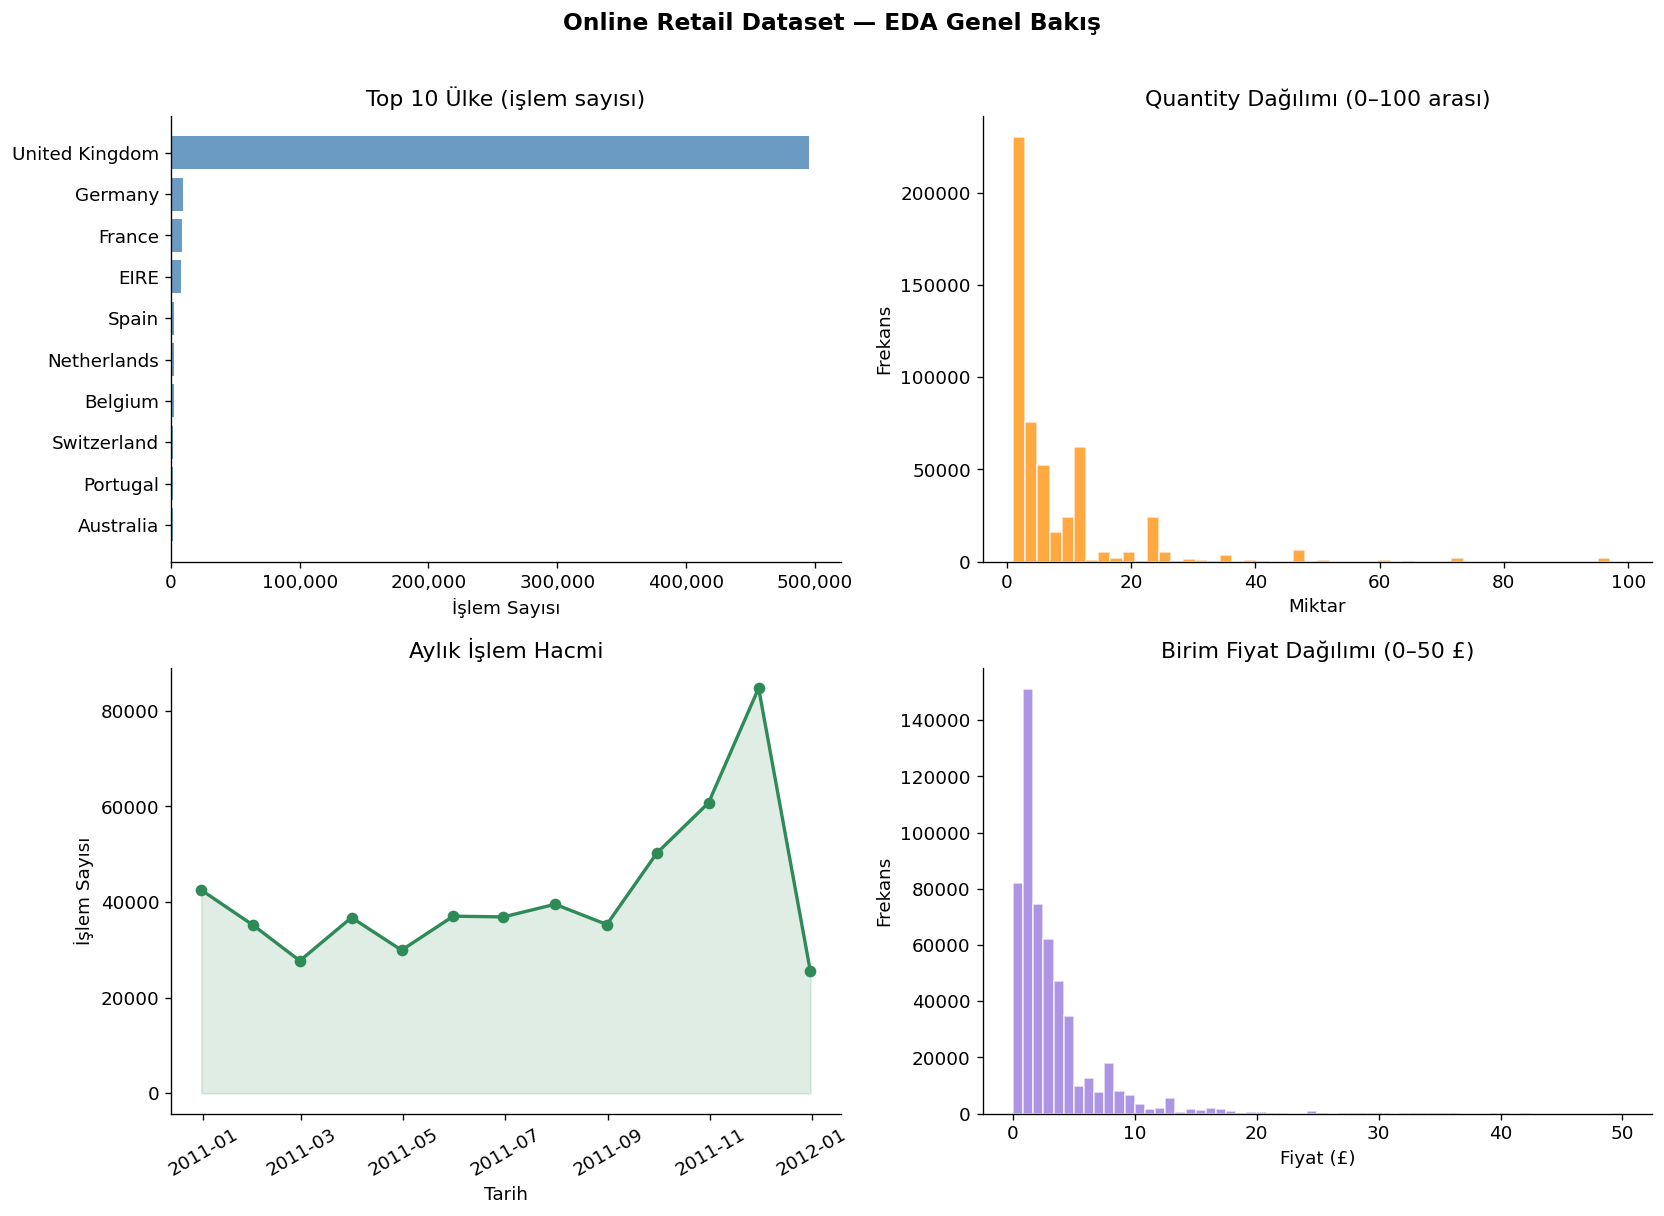
\includegraphics[width=0.85\textwidth]{eda_overview.png}}
    \caption{EDA overview: country distribution, quantity and price distributions, and monthly transaction volume.}
    \label{fig:eda}
\end{figure}

\begin{figure}[htbp]
    \centerline{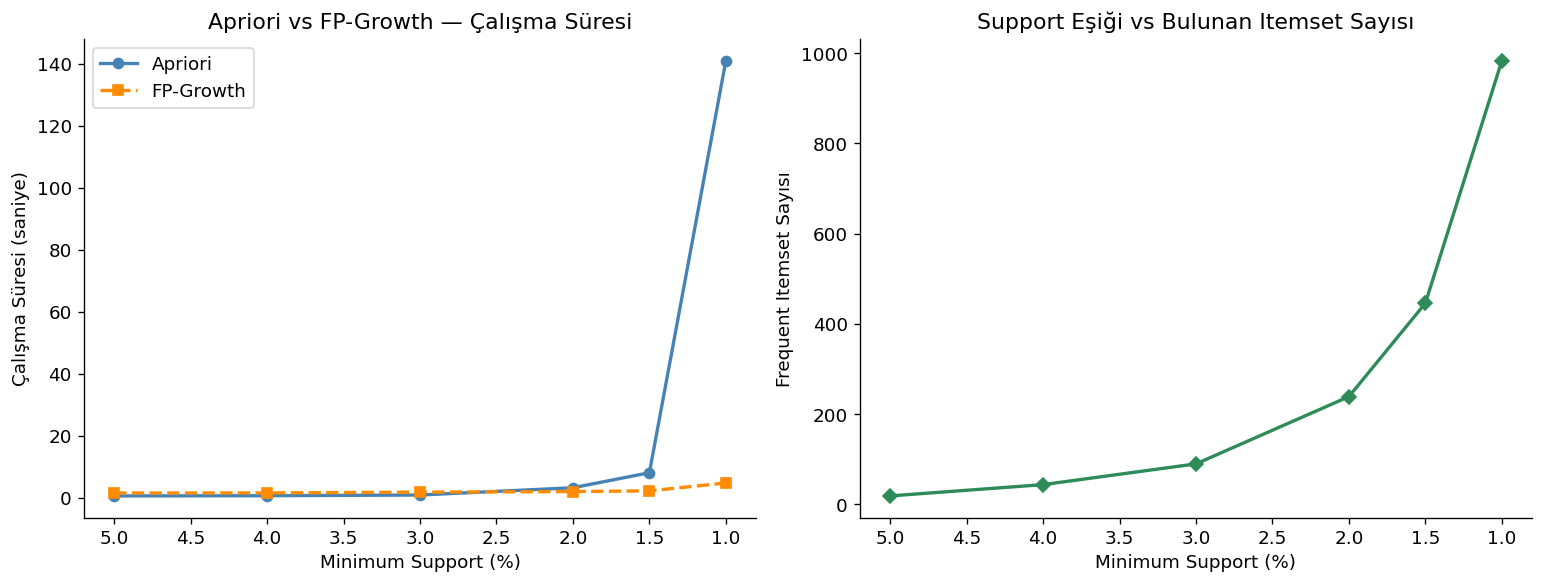
\includegraphics[width=0.85\textwidth]{apriori_vs_fpgrowth.png}}
    \caption{Left: Runtime comparison of Apriori and FP-Growth across support thresholds. Right: Number of frequent itemsets discovered vs. support threshold.}
    \label{fig:algos}
\end{figure}

\begin{figure}[htbp]
    \centerline{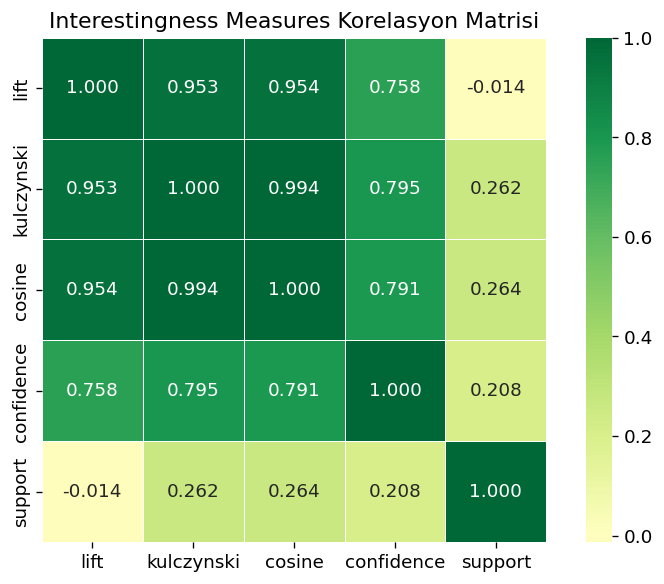
\includegraphics[width=0.6\textwidth]{measures_correlation.png}}
    \caption{Pearson correlation heatmap of interestingness measures. Kulczynski and cosine are highly correlated (r=0.994). Support shows near-zero correlation with lift.}
    \label{fig:corr}
\end{figure}

\end{document}
